\section{Background and Motivation}
\label{sec:background}

We briefly recall disk-based graph indexes and the usual ways of reducing their I/O, then show that those mechanisms still under-use each fetched page---already on the nearly uniform query set that ships with the benchmark.
Along the way we introduce the terms used in the rest of the paper and spell out the measurement behind Figure~\ref{fig:motivation_qps}.

\subsection{Disk Indexes, Node Caches, and Page Layouts}
In DiskANN-style systems~\cite{diskann}, compressed (product-quantized) vectors stay in DRAM while full-precision vectors and adjacency lists live on SSD, packed several nodes to a 4\,KB \emph{page}.
A query maintains a candidate list and repeatedly \emph{expands} the best unread candidate: it reads that node's page, scores its neighbors, and inserts promising ones into the list.
The candidate-list size $L$ and the beam width $W$ control how wide the walk is; larger $L$ or $W$ raises recall at the cost of more expansions and thus more random reads.
At billion scale a query often issues on the order of one hundred such reads, and I/O dominates latency.
Once a page is in memory, any later hop that lands on another node from that page costs no additional I/O; the challenge is to make such follow-on hits common.

A standard remedy is an in-memory \emph{node cache}: selected nodes are pinned in DRAM so that expanding them needs no SSD read.
DiskANN caches a BFS ball around the graph entry point; Laser~\cite{laser} favors high-in-degree nodes; run-time pools such as LRU track recent reads.
These policies differ in \emph{which} nodes they keep, but they share the same grain---full vector and adjacency of one node at a time, up to a DRAM budget.
They remove reads to the cached nodes themselves; they do little to decide which \emph{companions} should arrive with a node that still has to be fetched from SSD.

Starling~\cite{starling} and MARGO~\cite{margo} instead attack the on-disk layout: they reorder the index so that graph neighbors are more likely to share a page, and they search at page granularity.
The placement is computed from the graph (and, for MARGO, from construction-time path statistics) before serving, and then stays fixed.
That helps whenever the walk follows topology-local edges, but a page still holds only a handful of a node's dozens of neighbors, and the builder has no view of which of those edges a live query mix will actually use.
Existing work thus moves some nodes into memory early and improves the odds that a neighbor shares a page; what remains is to choose, from the query stream, which neighbors are worth bringing along on each miss---so that memory hits after the read cover more of the walk---without assuming that only heavily skewed traffic can benefit.

\subsection{N-Cache, D-Cache, and Seeds}
\label{sec:motivation}
We call the in-memory node cache the \emph{N-cache}: it stores hottest nodes at node grain under a DRAM budget (LRU in our measurements below).
Our second structure is an SSD-side \emph{D-cache}.
A D-cache entry is built around one graph node---the \emph{seed}---and stores that seed together with its neighbors (full vectors and adjacency for each), so that fetching the seed can also bring the nodes the walk is about to expand next.
How many 4\,KB pages that entry occupies depends on the seed's degree and on how many neighbors we choose to store; it is not fixed to a single page.
When those pages land in memory, later hops that hit the seed or a packed neighbor are ordinary DRAM hits.
D-cache does not invent a new hit domain and does not replace the base index: the search algorithm is unchanged, and D-cache entries are an extra on-SSD layout that stages more useful graph state per I/O.
N-cache and D-cache are complementary, not alternatives: the N-cache keeps the hottest vertices resident so they are never read from disk, while the D-cache makes each remaining SSD miss more productive by returning the seed together with neighbors the walk is likely to need next.

Because D-cache pages live on SSD, a miss still pays a disk read unless a recently fetched page is still in DRAM.
We therefore keep a small \emph{shared prefetch buffer}: a process-wide DRAM pool, shared by all search threads, that retains D-cache pages after they are read.
A later expansion---in the same query or in another thread---that needs a node on such a page hits the buffer and skips the SSD.
This buffer is not another node cache: it stores whole D-cache pages (seed plus packed neighbors) at page grain, and its only job is to avoid re-reading pages that were just brought in.
It is sized from the same DRAM budget as the N-cache so that enabling D-cache does not silently add memory.

The two LP bars in Figure~\ref{fig:motivation_qps} store every graph node as a seed together with \emph{all} of its neighbors---a \emph{full-neighborhood ceiling} that shows how large the packing gain can be when SSD cost is ignored.
\S\ref{sec:design} keeps the same idea---store a seed with neighbors beside it---but chooses which seeds to materialize and which neighbors to keep (the seed's \emph{hot edges}, made precise with the offline traces below), under an SSD budget.
Together, the N-cache and the budgeted D-cache form \textsc{NeighborCache}.

\begin{figure}[t]
  \centering
  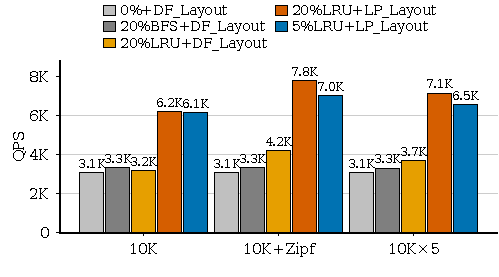
\includegraphics[width=\columnwidth]{figures/pub10k_workloads_grouped_qps.pdf}
  \caption{Throughput on SIFT100M (matched recall; $L{=}128$, $W{=}4$, 15 threads).
  Each name is the fraction of visited nodes in the node cache, then the page layout.
  DF\_Layout is DiskANN's default layout.
  LP\_Layout stores every node with all of its neighbors; those two bars also keep a 25\,MB prefetch of fetched LP pages.
  Left: the dataset's 10K queries; middle: mixed with Zipf draws; right: each query repeated $5\times$.}
  \label{fig:motivation_qps}
  \Description{Grouped bar chart of QPS on SIFT100M for five cache-and-layout settings under the dataset 10K queries, a Zipf mix, and five-fold repetition.}
\end{figure}

\subsection{A Full-Neighborhood Ceiling on the Dataset Query Set}
Figure~\ref{fig:motivation_qps} is a controlled comparison on SIFT100M under DiskANN search with $L{=}128$, $W{=}4$, and 15 threads.
We report throughput (queries per second, QPS) at matched recall: every bar uses the same search parameters so that quality stays aligned and the differences come from caching and page contents, not from a looser walk.
The percentage is the fraction of nodes visited by these searches that the node cache holds.
DF\_Layout is DiskANN's default page layout.
LP\_Layout is the full-neighborhood ceiling: every node is a seed and stores all of its neighbors.
The two LP bars also keep a 25\,MB shared prefetch of fetched LP pages; that buffer is not part of the percentage.
The five bars are: (i)~0\%+DF\_Layout, plain DiskANN with no node cache; (ii)~20\%BFS+DF\_Layout, an entry-point BFS cache of that fraction on the default layout; (iii)~20\%LRU+DF\_Layout, an LRU cache of that fraction on the default layout; (iv)~20\%LRU+LP\_Layout and (v)~5\%LRU+LP\_Layout, the same LRU policy on the full-neighborhood layout.
The leftmost group is the 10K query set that accompanies SIFT100M, which is close to uniform over the index.
The middle group concatenates that 10K with another 10K drawn Zipf-skewed ($\alpha{=}0.8$) and shuffles the mix, so some queries repeat more often without changing the underlying index.
The right group repeats each of the original 10K queries five times (shuffled), a simple repetitive workload.
0\%+DF\_Layout and 20\%BFS+DF\_Layout stay near 3.1K--3.3K~QPS in all three groups.
20\%LRU+DF\_Layout does little better on the dataset's 10K (3.2K) and reaches 4.2K under Zipf and 3.7K under five-fold repetition.
On the full-neighborhood layout, 20\% LRU reaches 6.2K~QPS on that 10K---about twice DiskANN---and 7.8K and 7.1K under Zipf and five-fold repetition.
Cutting the LRU from 20\% to 5\% of visited nodes leaves 6.1K, 7.0K, and 6.5K~QPS.
Production traffic is often skewed, and that helps; the important reading is that the dataset's own query set was already enough to show a large gap.

After a D-cache miss, the fetched pages land in DRAM, so expansions that find the seed or a packed neighbor there need no further I/O.
A conventional node cache typically pays for one vertex at a time; a D-cache entry pays for the seed plus neighbors the walk is likely to take next, so the transfer can cover a short path segment.
Graph traversal reuses local structure even when query IDs look uniform, which is why the left cluster in Figure~\ref{fig:motivation_qps} moves at all: the gain is not from query-ID skew alone, but from packing the neighbors the walk actually follows.

\subsection{From Ceiling to NeighborCache}
Storing every node's full neighborhood in Figure~\ref{fig:motivation_qps} is easy to measure and expensive to keep: the extra SSD footprint is already tens of times the disk index on SIFT100M-scale data, before counting refresh work.
\S\ref{sec:design} therefore materializes only a budgeted subset of seeds, stores beside each seed the neighbors reached through its hot edges rather than every neighbor, updates those entries without stalling search, and retires them as popularity drifts, while leaving the base index untouched.

Offline traces on SIFT1B support the same conclusion with access counts rather than QPS.
SSD reads concentrate on a small set of \emph{hot nodes}; an entry-point BFS cache covers little of that set.
For each hot node, only a few of its many outgoing edges are taken repeatedly by searches\todo{fill top-$k$ / coverage}; we call those edges \emph{hot edges}.
A practical D-cache entry should store, beside the seed, the neighbors reached through those hot edges---not an arbitrary topology neighborhood.
Starling and MARGO decide co-location from the graph (or from construction-time path weights) and therefore do not observe these query-driven edges; that gap is why topology layouts leave the miss cost of Figure~\ref{fig:motivation_qps} largely intact, while packing the edges that searches actually follow raises QPS already on the dataset's 10K queries.

\textsc{NeighborCache} implements this under an SSD budget: hottest nodes in the N-cache, a bounded set of seed-and-neighbor D-cache entries maintained from online searches, and no change to the base index or search algorithm.
